\section{Herstellung der ersten Platine}

\subsection{Entwurf einer Leiterplatte}
Zum Entwurf einer funktionsfähigen Platine sind ein Schaltplan, ein PCB-Layout und die passenden Bauteile mit zugehörigen Footprints erforderlich.
Für die erste Platine werden nur Testpunkte erstellt, weshalb die Erstellung eigener Bauteile und Footprints in sogenannten Libraries nicht im Fokus stand.
Der Schwerpunkt liegt vielmehr auf der Herstellung einer spezifischen Leiterbahn mit auf der Platine.\\
\\
Eine besondere Anforderung bestand darin, eine Leiterbahn mit einem definierten Widerstand von genau $200,\text{m}\Omega$ zu realisieren.
Um dies zu erreichen wird eine feste Breite für die Leiterbahn vorgegeben, anhand derer die erforderliche Länge der Bahn berechnet werden muss.

\paragraph{Berechnung:} 
\begin{align*}
\text{Gegeben:} & \quad b=0{,}275\,\text{mm}, \quad R=0{,}2\,\Omega, \quad \rho=0{,}01721\,\Omega\cdot\text{mm}^2/\text{m}, \quad h=0{,}035\,\text{mm} \\ 
\text{Gesucht:} & \quad l \\ R &= \frac{\rho \cdot l}{A} \quad \Rightarrow \quad l = \frac{R \cdot b \cdot h}{\rho} \\
l &= \frac{0{,}2\,\Omega \cdot 0{,}275\,\text{mm} \cdot 0{,}035\,\text{mm}}{0{,}01721\,\Omega\cdot\text{mm}^2/\text{m}} = 111{,}85\,\text{mm} 
\end{align*}
\\
Die berechnete Länge wird anschließend in das Platinenlayout erstellt.
Da die Gesamtlänge der Leiterbahn durch das Layout die berechneten Länge überschreiten könnte, wird die Leiterbahn in einem wellenartigen Muster umgesetzt, um die geforderte Gesamtlänge einzuhalten.

\begin{figure}[h]
\centering 
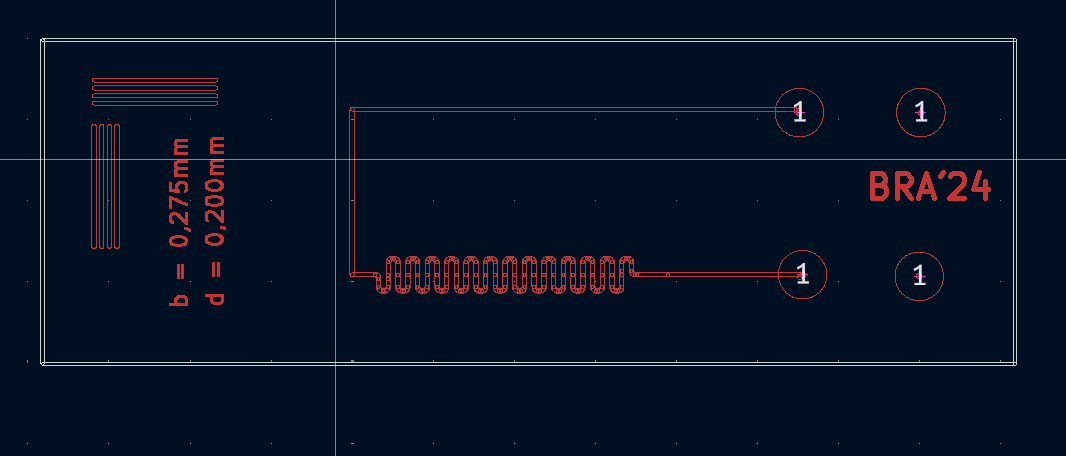
\includegraphics [width=\linewidth, height=6cm]{\figdir/PCB-Layout breite 0,275mm.png}
\caption{PCB Layout der Platine mit Leiterbahn = 0,275 mm}
\label{fig:Abbildung 1}
\end{figure}

\noindent
Außerdem wird der Name des Studierenden zusammen mit der Jahreszahl auch als Kupferbahn ausgeführt.
Bei der herkömmlichen Fertigung von Leiterplatten wird ein Bestückungsdruck für Bezeichnung der Komponenten und zusätzlichen Informationen zu den Bauteilen verwendet.
Da hier allerdings nur eine Kupferschicht vorgesehen ist, wird darauf verzichtet.
\\
Für die nachfolgende Messung bzw. Überprüfung unter dem Mikroskop werden vier Linien horizontal und vertikal in festem Abstand auf der Leiterplatte definiert.





\subsection{Herstellung der Platine}
Zur Herstellung von Platinen gibt es verschiedenste Verfahren. An der Hochschule werden die Platinen mittels eines Ätzverfahrens hergestellt. Dieses Verfahren besteht im Wesentlichen aus drei Schritten: dem Belichten, Entwickeln und Ätzen.

\subsubsection{Belichten}
Beim Ätzverfahren befindet sich auf der Platine ein Ätzresistlack. Dieser Lack muss mit Hilfe von Belichten an bestimmten Stellen seine Wirkung verlieren. \ldots

\subsubsection{Entwickeln}
Für die Entwicklung der Platine wird diese in einen Rahmen eingespannt und anschließend in eine Kammer gehängt. In dieser Kammer wird der Rohling mit Natronlauge besprüht. \ldots

\subsubsection{Ätzen}
Zum Ätzen der Platine wird diese wieder in einen Rahmen gespannt und anschließend in einer Kammer mit Eisen-III-Chlorid besprüht. \ldots
